% Chapter Template

\chapter{Test Problems and Models} % Main chapter title

\label{Chapter4}

\lhead{Chapter 4. \emph{Test Problems and Models}} 

For the purpose of testing the KLT as a basis generator for the ERMM, a number 
of test problems and corresponding snapshot models were developed. A total of 
three test problems were constructed, two that are 1-D and one that is 2-D.  
These test problems serve as the way to benchmark the implementation of 
KLT into the ERMM as a way to approximate the energy variable.

\section{Test Problems}

The test problems considered are (1) a 1-D, 10-pin, UO$_2$-MOX 
assembly model, (2) a 1-D, 70-pin BWR core model, and (3) the 2-D C5G7 benchmark
\citep{C5G7}. The transport code DETRAN was used with a 16-angle, 
double Gauss-Legendre quadrature and a step-characteristic spatial 
discretization for problems (1) and (2). Problem (3) was solved with a  
Gauss-Chebyshev quadrature for the polar variable and Abu-Shumays' 
Quadruple Range quadrature for the azimuthal variable \citep{Roberts2014}. 
Cross-section libraries for the test problems were generated with SCALE 6.1 in 
the SCALE 44-group and 238-group formats \citep{Scale}.

For the 1-D problems, a current-conserving, first-order, angular expansion 
based on Jacobi polynomials \citep{Roberts2014} was used.  For the 2-D 
problem, a set of Chebyshev polynomials was used for the angular expansion. For 
the 1-D problems, nodal boundary currents have no spatial dependence thereby 
rendering spatial expansions unnecessary, but for the 2-D problem, a spacial 
expansion based on DLP was used. For energy, DLP, mDLP, and KLT bases were 
explored as a function of the energy expansion order.

All calculations were performed with the SERMENT parallel response matrix 
code \citep{RobertsSerment}, which links to the DETRAN deterministic 
transport code \citep{RobertsDetran}.  To implement each of the test problems, 
each was first solved in DETRAN to provide the snapshots (which are 
discussed later in this chapter).  Next, each model was solved again using 
SERMENT for the full multi-group reference case.  The same spatial and angular 
expansion order was used throughout the calculations for each test problem and 
corresponding snapshot models. Finally, SERMENT was used to calculate the 
test problem for several expansion orders with the chosen basis set.  These 
calculations were compared to the reference case, and the results are presented 
in \CHAPTER{Chapter5} for the 1-D problems and \CHAPTER{Chapter6} for the 2-D 
problem.

\subsection{1-D Test Problems}

Two 1-D test problems were developed.  The first, the 10-pin problem, serves as 
the proof of concept.  It was a relatively simple problem to show how KLT can be used to 
approximate the junction between two fuel types with very different spectral 
properties.  The second problem is designed to be more complex and, thus, more 
difficult to model.  It is a 1-D, full-core model with several fuel assembly types, and, due to its 
complexity, it should provide a better test of KLT.

\subsubsection*{10-Pin Problem}

The first test problem was a 1-D approximation to the junction between a UO$_2$  
and MOX assembly. In the 10-pin test problem, fuel for the left five pins was 
4\% enriched UO$_2$, while the right five pins were composed of 
4.3\% enriched MOX (The fuel contained 4.3\% plutonium with the remainder 
natural uranium), as shown in  
\FIG{fig:10-pin_config}. Boundary conditions on either side of the model were 
reflective. 

\begin{figure*}[htb]
    \centering
    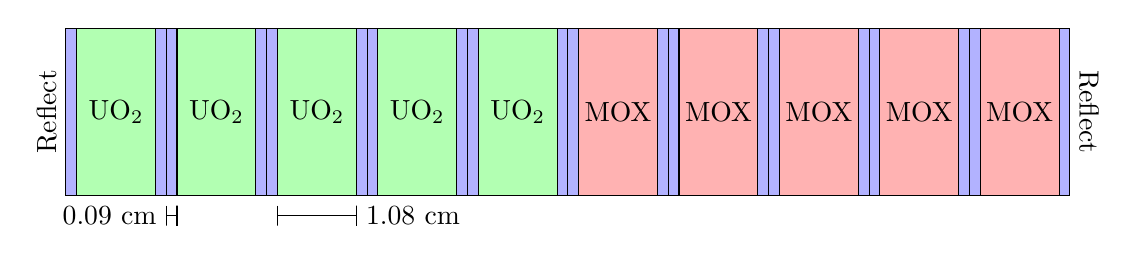
\begin{tikzpicture}[scale=0.85, every node/.style={scale=1}]
        \foreach \x in {0,1.5,...,6}
        \filldraw[xshift=\x cm, fill=green!30!white, draw=black] (0.160714286,0) 
        rectangle (1.339285714,2.5) node[pos=.5] {UO$_2$};
        \foreach \x in {7.5,9,...,13.5}
        \filldraw[xshift=\x cm, fill=red!30!white, draw=black] (0.160714286,0) 
        rectangle (1.339285714,2.5) node[pos=.5] {MOX};
        \foreach \x in {0,1.5,...,13.5}
        \filldraw[xshift=\x cm, fill=blue!30!white, draw=black] (0,0) rectangle 
        (0.160714286,2.5);
        \foreach \x in {0,1.5,...,13.5}
        \filldraw[xshift=\x cm, fill=blue!30!white, draw=black] (1.339285714,0) 
        rectangle (1.5,2.5);
        \draw[xshift=15cm,yshift=1.25cm] node[right] {\rotatebox{-90}{Reflect}};
        \draw[yshift=1.25cm] node[left] {\rotatebox{90}{Reflect}};
        \draw (1.5,-.15) -- (1.5,-.45) -- (1.5,-.30) node[left] {0.09 cm} -- 
        (1.660714286,-.30) -- (1.660714286,-.15) -- (1.660714286, -.45);
        \draw (3.160714286,-.15) -- (3.160714286,-.45) -- (3.160714286,-.30) -- 
        (4.339285714,-.30) node[right] {1.08 cm} -- (4.339285714,-.15) -- 
        (4.339285714, -.45);
    \end{tikzpicture}
    \caption{Configuration for 10-pin Test Problem}
    \label{fig:10-pin_config}
\end{figure*}

Fuel pins were 1.08 cm thick with 0.09 cm of moderator on each side. The 
baseline pincell discretization consisted of 22 mesh cells of fuel enclosed by 
three mesh cells of moderator on either side; therefore, each pincell provided
28 energy-dependent snapshots.

Because the test problem reference solution is a full transport approximation, 
boundary currents generally exhibit coupled angle-energy dependence.  By 
including snapshots that incorporate angular information, the resulting KLT 
basis set
may outperform snapshots based only on the energy-dependent scalar flux $\phi$. 
 To include angular information, snapshots were taken of the energy-dependent 
partial current $J_{\text{left}}$. Snapshots of the net current were previously 
considered, but those snapshots performed as well as or worse than the partial 
current in all cases.  Further, because the snapshot models were symmetric, the 
direction of the partial current is selected arbitrarily. Finally, because the
spatial discretization produces only 
one spatial unknown per cell, the snapshot generation approach used provided 
one 
($\phi$ or $J_{\text{left}}$) or two ($\phi$ and $J_{\text{left}}$) snapshots 
per spatial cell.

In addition to inclusion of snapshots of the partial current for each test 
problem, 
the addition of snapshots of higher-order angular moments was studied.  These 
moments were generated by expanding the angular flux $\psi$ through a Jacobi 
expansion in angle.  In this basis, the zeroth moment is equivalent to the 
partial current, while higher moments have less well-defined physical corollaries.  
Inclusion of these moments (up through second order) was studied for both test 
problems and are presented at the end of the results section.

Several combinations for the snapshot types were considered and presented in 
the following chapters.  First, snapshots of just $\phi$ were used.  Second, 
snapshots of just $J_{\text{left}}$ were used.  Third, KLT was used 
with snapshots of both $\phi$ and $J_{\text{left}}$ together.  Fourth, snapshots 
of each of the 
higher order moments (up through order two) were used individually for the test 
problems (e.g., snapshots from just angular moment two).  Finally, The 
snapshots for $\phi$, $J_{\text{left}}$, and the higher moments (incrementing 
upward in order) were used for basis generation (e.g., $\phi$, 
$J_{\text{left}}$, 
order 1 or $\phi$, $J_{\text{left}}$, order 1, order 2 etc.).

\subsubsection*{BWR Test Problem}

The second test case, representative of a boiling water reactor (BWR), was 
comprised of seven assemblies, each with 10 pins.  Three core configurations 
were used, and each core configuration had two unique assemblies.  Three fuel 
types were used, including 4.5\% enriched UO$_2$, 2.5\% enriched UO$_2$, and 
4.5\% enriched UO$_2$ with 5 wt\% Gd$_2$O$_3$.  Core and assembly 
configurations 
are shown in \FIG{fig:BWRconfig}. Boundary conditions for this case were 
vacuum.  This test problem was adapted from the work of \citet{Nichita1998} and 
\citet{Ilas2003}.
\begin{figure*}[htb]
    \begin{minipage}[c]{\textwidth}
        \centering
        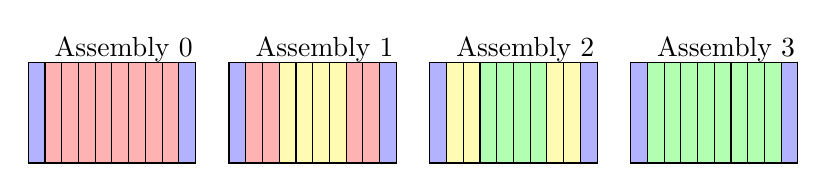
\begin{tikzpicture}[scale=0.85, every node/.style={scale=1}]
            \foreach \x in {0,2.25,3,5.25,6,8.25,9,11.25}
            \filldraw[xshift=\x cm,fill=blue!30!white,draw=black] (0,0) 
            rectangle (0.25,1.5);
            \foreach \x in {.25,.5,.75,1,1.25,1.5,1.75,2,3.25,3.5,4.75,5}
            \filldraw[xshift=\x cm,fill=red!30!white,draw=black] (0,0) 
            rectangle (0.25,1.5);
            \foreach \x in {3.75,4,4.25,4.5,6.25,6.5,7.75,8}
            \filldraw[xshift=\x cm,fill=yellow!30!white,draw=black] (0,0) 
            rectangle (0.25,1.5);
            \foreach \x in 
            {6.75,7,7.25,7.5,9.25,9.5,9.75,10,10.25,10.5,10.75,11}
            \filldraw[xshift=\x cm,fill=green!30!white,draw=black] (0,0) 
            rectangle (0.25,1.5);
            \draw (0.25,1.7) node[right] {Assembly 0};%
            \draw (3.25,1.7) node[right] {Assembly 1};%
            \draw (6.25,1.7) node[right] {Assembly 2};%
            \draw (9.25,1.7) node[right] {Assembly 3};%
        \end{tikzpicture}
    \end{minipage} 
    \begin{minipage}[c]{\textwidth}
        \centering
        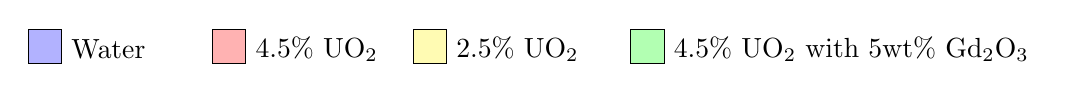
\begin{tikzpicture}[scale=0.85, every node/.style={scale=1}]
            \filldraw[xshift=-4cm,fill=blue!30!white,draw=black] (-.25,-.25) 
            rectangle (.25,.25) node[yshift=-.25cm, right] {Water};%
            \filldraw[xshift=-1.25cm,fill=red!30!white,draw=black] (-.25,-.25) 
            rectangle (.25,.25) node[yshift=-.25cm, right] {4.5$\%$ UO$_2$};%
            \filldraw[xshift=1.75cm,fill=yellow!30!white,draw=black] 
            (-.25,-.25) rectangle (.25,.25) node[yshift=-.25cm, 
            right] {2.5$\%$ UO$_2$};%
            \filldraw[xshift=5cm,fill=green!30!white,draw=black] (-.25,-.25) 
            rectangle (.25,.25) node[yshift=-.25cm, right] {4.5$\%$ UO$_2$ with 
            5wt$\%$ Gd$_2$O$_3$};%
        \end{tikzpicture}
    \end{minipage}
    \begin{minipage}[c]{\textwidth}
        \centering
        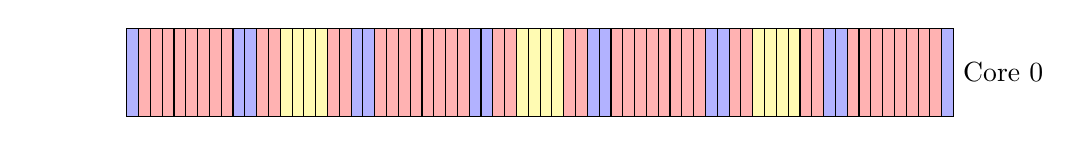
\begin{tikzpicture}[scale=1.5, every node/.style={scale=1}]
            \foreach \x in {0,.1,...,6.9}
            \filldraw[xshift=\x cm,fill=red!30!white,draw=black] (0,0) 
            rectangle (0.1,.75);
            \foreach \x in {0,1,2,3,4,5,6,.9,1.9,2.9,3.9,4.9,5.9,6.9}
            \filldraw[xshift=\x cm,fill=blue!30!white,draw=black] (0,0) 
            rectangle (0.1,.75);
            \foreach \x in {1.3,1.4,1.5,1.6,3.3,3.4,3.5,3.6,5.3,5.4,5.5,5.6}
            \filldraw[xshift=\x cm,fill=yellow!30!white,draw=black] (0,0) 
            rectangle (0.1,.75);
            \draw (7,.375) node[right] {Core 0};%
            \draw (0,.375) node[left,color=white] {Core 0};
        \end{tikzpicture}
    \end{minipage}
    \begin{minipage}[c]{\textwidth}
        \centering
        \vspace*{.15cm}
        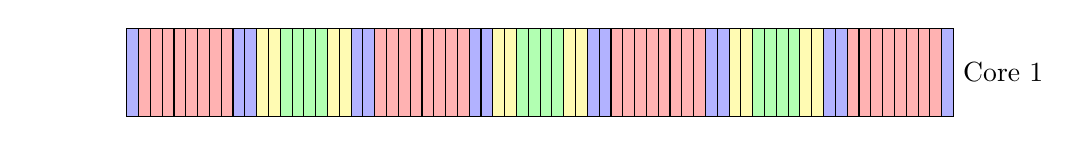
\begin{tikzpicture}[scale=1.5, every node/.style={scale=1}]
            \foreach \x in {0,.1,...,6.9}
            \filldraw[xshift=\x cm,fill=red!30!white,draw=black] (0,0) 
            rectangle (0.1,.75);
            \foreach \x in {0,1,2,3,4,5,6,.9,1.9,2.9,3.9,4.9,5.9,6.9}
            \filldraw[xshift=\x cm,fill=blue!30!white,draw=black] (0,0) 
            rectangle (0.1,.75);
            \foreach \x in {1.1,1.2,1.7,1.8,3.1,3.2,3.7,3.8,5.1,5.2,5.7,5.8}
            \filldraw[xshift=\x cm,fill=yellow!30!white,draw=black] (0,0) 
            rectangle (0.1,.75);
            \foreach \x in {1.3,1.4,1.5,1.6,3.3,3.4,3.5,3.6,5.3,5.4,5.5,5.6}
            \filldraw[xshift=\x cm,fill=green!30!white,draw=black] (0,0) 
            rectangle (0.1,.75);
            \draw (7,.375) node[right] {Core 1};%
            \draw (0,.375) node[left,color=white] {Core 1};
        \end{tikzpicture}
    \end{minipage}
    \begin{minipage}[c]{\textwidth}
        \centering
        \vspace*{.15cm}
        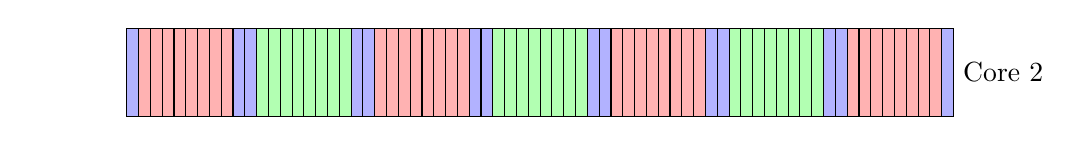
\begin{tikzpicture}[scale=1.5, every node/.style={scale=1}]
            \foreach \x in {0,.1,...,6.9}
            \filldraw[xshift=\x cm,fill=red!30!white,draw=black] (0,0) 
            rectangle (0.1,.75);
            \foreach \x in {0,1,2,3,4,5,6,.9,1.9,2.9,3.9,4.9,5.9,6.9}
            \filldraw[xshift=\x cm,fill=blue!30!white,draw=black] (0,0) 
            rectangle (0.1,.75);
            \foreach \x in {1.1,1.2,1.3,1.4,1.5,1.6,1.7,1.8, 
                            3.1,3.2,3.3,3.4,3.5,3.6,3.7,3.8,
                            5.1,5.2,5.3,5.4,5.5,5.6,5.7,5.8}
            \filldraw[xshift=\x cm,fill=green!30!white,draw=black] (0,0) 
            rectangle (0.1,.75);
            \draw (7,.375) node[right] {Core 2};%
            \draw (0,.375) node[left,color=white] {Core 2};
        \end{tikzpicture}
    \end{minipage}
    \caption{Configuration for BWR Test Problem}
    \label{fig:BWRconfig}
\end{figure*}  

Fuel pins for the second problem were 0.72 cm thick with 0.27 cm of moderator 
on each side. The baseline pincell discretization consisted of 16 mesh cells of 
fuel enclosed by six mesh cells of moderator; therefore, each pincell provided 
28 energy-dependent snapshots. With 70 pincells, the total number of snapshots 
was 1960, but the right set of snapshots was identical to the left with respect 
to scalar flux due to symmetry.  For these simple 1-D problems, finer spatial and angular 
refinement was unnecessary.

For the BWR test problem, the combinations of potential 
snapshots were the same as used for the 10-pin test problem; however the snapshot models 
used to 
generate snapshots were different, as will be discussed later in this chapter.

\subsection{2-D Test Problems}

The C5G7 benchmark is a well-studied problem for assessing numerical methods in 
neutron transport and reactor physics. This benchmark consists of modeling a 
quarter core that has four, $17\times17$-pin 
assemblies \citep{C5G7}.  The configuration is detailed in  
\FIG{fig:C5G7_config}.  Each of the blocks in \FIG{fig:C5G7_config} 
represent either a fuel assembly or an equivalent area of 
moderator.  The configuration of the UO$_2$ assembly is shown in  
\FIG{fig:UO2_config} and the configuration of the MOX bundle is shown in  
\FIG{fig:MOX_config}.  Each individual pincell is modeled as shown in  
\FIG{fig:pin_cell_config}. Each pincell is broken up into a $7\times7$ 
Cartesian 
mesh. Thus each pincell contained 49 spatial cells and provided 49 energy 
dependent snapshots of each type.  The cladding for the pincells was 
homogenized into the fuel part of the pincell.  

\begin{figure*}[htb]
    \centering
    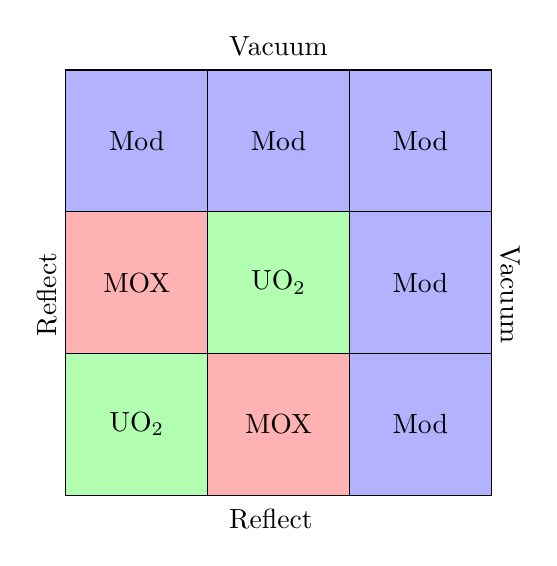
\begin{tikzpicture}[scale=0.6, every node/.style={scale=1}]
        \filldraw[xshift=6 cm, yshift=0 cm, fill=blue!30!white, draw=black] 
        (0, 0) rectangle (3,3) node[pos=.5] {Mod};
        \filldraw[xshift=6 cm, yshift=3 cm, fill=blue!30!white, draw=black] 
        (0, 0) rectangle (3,3) node[pos=.5] {Mod};
        \filldraw[xshift=6 cm, yshift=6 cm, fill=blue!30!white, draw=black] 
        (0, 0) rectangle (3,3) node[pos=.5] {Mod};
        \filldraw[xshift=3 cm, yshift=6 cm, fill=blue!30!white, draw=black] 
        (0, 0) rectangle (3,3) node[pos=.5] {Mod};
        \filldraw[xshift=0 cm, yshift=6 cm, fill=blue!30!white, draw=black] 
        (0, 0) rectangle (3,3) node[pos=.5] {Mod};
        \filldraw[xshift=0 cm, yshift=0 cm, fill=green!30!white, draw=black] 
        (0, 0) rectangle (3,3) node[pos=.5] {UO$_2$};
        \filldraw[xshift=3 cm, yshift=3 cm, fill=green!30!white, draw=black] 
        (0, 0) rectangle (3,3) node[pos=.5] {UO$_2$};
        \filldraw[xshift=3 cm, yshift=0 cm, fill=red!30!white, draw=black] 
        (0, 0) rectangle (3,3) node[pos=.5] {MOX};
        \filldraw[xshift=0 cm, yshift=3 cm, fill=red!30!white, draw=black] 
        (0, 0) rectangle (3,3) node[pos=.5] {MOX};
        \draw[xshift=9cm,yshift=4.25cm] node[right] 
        {\rotatebox{-90}{Vacuum}};
        \draw[yshift=4.25cm] node[left] {\rotatebox{90}{Reflect}};
        \draw[xshift=3.25cm,yshift=9.5cm] node[right] {{Vacuum}};
        \draw[xshift=3.25cm, yshift=-.5cm] node[right] {{Reflect}};
    \end{tikzpicture}
    \caption{Configuration for Full-Core.  Each square represents the area of a 
             $17\times17$ pin assembly}
    \label{fig:C5G7_config}
\end{figure*}

\begin{figure*}[htb]
    \centering
    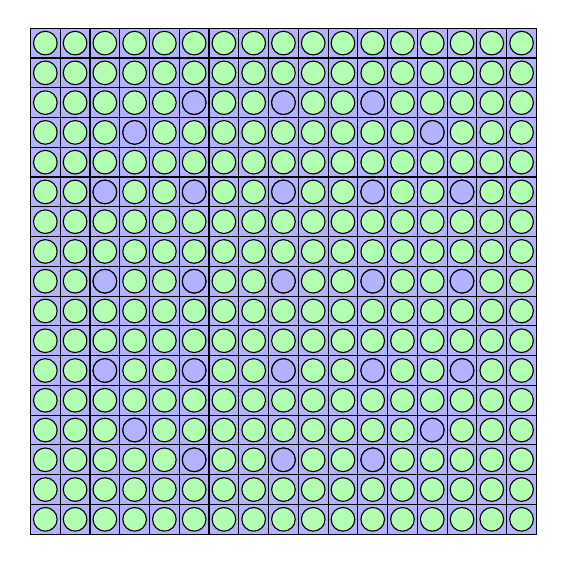
\begin{tikzpicture}[scale=0.3, every node/.style={scale=1}]
        \foreach \x in {0,1.26,...,20.16}
        \foreach \y in {0,1.26,...,20.16}
        \filldraw[xshift=\x cm, yshift=\y cm, fill=blue!30!white, 
        draw=black] (0, 0) rectangle (1.26,1.26) node[pos=.5] {};
        \foreach \x in {0,1.26,...,20.16}
        \foreach \y in {0,1.26,...,20.16}
        \filldraw[xshift=\x cm, yshift=\y cm, fill=green!30!white, 
        draw=black] (.63,.63) circle (.5) node[pos=.5] {};
        \foreach \x in {5*1.26, 8*1.26, 11*1.26}
        \foreach \y in {2*1.26, 14*1.26}
        \filldraw[xshift=\x cm, yshift=\y cm, fill=blue!30!white, 
        draw=black] (.63,.63) circle (.5) node[pos=.5] {};
        \foreach \x in {3*1.26, 13*1.26}
        \foreach \y in {3*1.26, 13*1.26}
        \filldraw[xshift=\x cm, yshift=\y cm, fill=blue!30!white, 
        draw=black] (.63,.63) circle (.5) node[pos=.5] {};
        \foreach \x in {2*1.26, 5*1.26, 8*1.26, 11*1.26, 14*1.26}
        \foreach \y in {5*1.26, 8*1.26, 11*1.26}
        \filldraw[xshift=\x cm, yshift=\y cm, fill=blue!30!white, 
        draw=black] (.63,.63) circle (.5) node[pos=.5] {};
    \end{tikzpicture}
    \caption{Configuration for UO$_2$ fuel bundle.  The green represents a 
             UO$_2$ pincell, while the blue represents a guide tube modeled as 
             a pincell filled with moderator}
    \label{fig:UO2_config}
\end{figure*}
\begin{figure*}[htb]
    \centering
    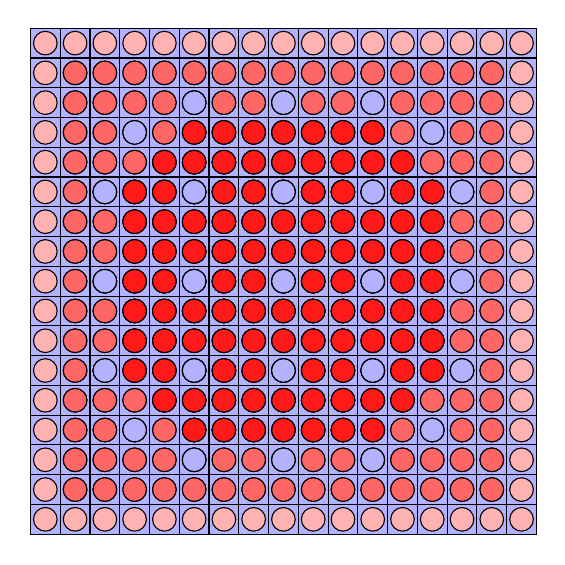
\begin{tikzpicture}[scale=0.3, every node/.style={scale=1}]
        \foreach \x in {0,1.26,...,20.16}
        \foreach \y in {0,1.26,...,20.16}
        \filldraw[xshift=\x cm, yshift=\y cm, fill=blue!30!white, 
        draw=black] (0, 0) rectangle (1.26,1.26) node[pos=.5] {};
        \foreach \x in {0,1.26,...,20.16}
        \foreach \y in {0,1.26,...,20.16}
        \filldraw[xshift=\x cm, yshift=\y cm, fill=red!30!white, draw=black] 
        (.63,.63) circle (.5) node[pos=.5] {};
        \foreach \x in {1.26,2.52,...,20.16}
        \foreach \y in {1.26,2.52,...,20.16}
        \filldraw[xshift=\x cm, yshift=\y cm, fill=red!60!white, draw=black] 
        (.63,.63) circle (.5) node[pos=.5] {};
        \foreach \x in {5*1.26,6*1.26,7*1.26,8*1.26,9*1.26,10*1.26,11*1.26}
        \foreach \y in {3*1.26,13*1.26}
        \filldraw[xshift=\x cm, yshift=\y cm, fill=red!90!white, draw=black] 
        (.63,.63) circle (.5) node[pos=.5] {};
        \foreach \x in 
        {4*1.26,5*1.26,6*1.26,7*1.26,8*1.26,9*1.26,10*1.26,11*1.26,12*1.26}
        \foreach \y in {4*1.26,12*1.26}
        \filldraw[xshift=\x cm, yshift=\y cm, fill=red!90!white, draw=black] 
        (.63,.63) circle (.5) node[pos=.5] {};
        \foreach \x in {3.78,5.04,...,16.38}
        \foreach \y in {6.3,7.56,...,15.04}
        \filldraw[xshift=\x cm, yshift=\y cm, fill=red!90!white, draw=black] 
        (.63,.63) circle (.5) node[pos=.5] {};
        \foreach \x in {5*1.26, 8*1.26, 11*1.26}
        \foreach \y in {2*1.26, 14*1.26}
        \filldraw[xshift=\x cm, yshift=\y cm, fill=blue!30!white, 
        draw=black] (.63,.63) circle (.5) node[pos=.5] {};
        \foreach \x in {3*1.26, 13*1.26}
        \foreach \y in {3*1.26, 13*1.26}
        \filldraw[xshift=\x cm, yshift=\y cm, fill=blue!30!white, 
        draw=black] (.63,.63) circle (.5) node[pos=.5] {};
        \foreach \x in {2*1.26, 5*1.26, 8*1.26, 11*1.26, 14*1.26}
        \foreach \y in {5*1.26, 8*1.26, 11*1.26}
        \filldraw[xshift=\x cm, yshift=\y cm, fill=blue!30!white, 
        draw=black] (.63,.63) circle (.5) node[pos=.5] {};
    \end{tikzpicture}
    \caption{Configuration for MOX bundle.  The light red represents 4.3\% MOX 
             fuel, the medium red represents 7.0 \% MOX fuel, and the dark red 
             represents 8.7\% MOX fuel.  The blue represents moderator (i.e.,  
             light water)}
    \label{fig:MOX_config}
\end{figure*}
\begin{figure*}[htb]
    \centering
    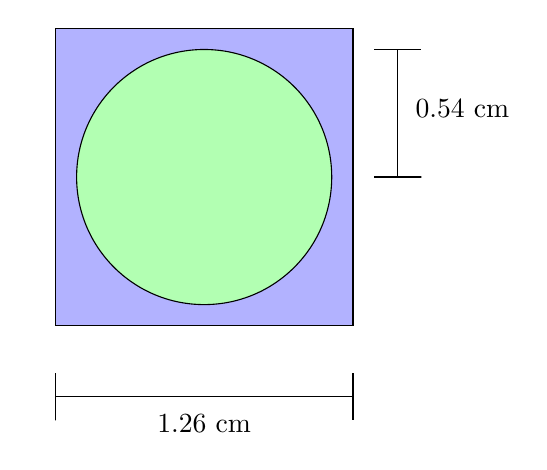
\begin{tikzpicture}[scale=3, every node/.style={scale=1}]
        \filldraw[xshift=0 cm, yshift=0 cm, fill=blue!30!white, draw=black] 
        (0, 0) rectangle (1.26,1.26) node[pos=.5] {};
        \filldraw[xshift=0 cm, yshift=0 cm, fill=green!30!white, draw=black] 
        (.63,.63) circle (.54) node[pos=.5] {};
        \draw (0,-.2) -- (0,-.4) -- (0,-.30) -- (0.63,-.3) node[below=0.1cm] 
        {1.26 cm} -- (1.26,-.30) -- (1.26,-.2) -- (1.26, -.4);
        \draw (1.35,.63) -- (1.55,.63) -- (1.45,.63) -- (1.45,.92) 
        node[right=0.1cm] {0.54 cm} -- (1.45,1.17) -- (1.35,1.17) -- (1.55, 
        1.17);
    \end{tikzpicture}
    \caption{Configuration for pincell.  The circular fuel element had a 
             radius of 0.54 cm and was homogenized with cladding for this 
             model.}
    \label{fig:pin_cell_config}
\end{figure*}

Although the original C5G7 benchmark was defined with 7-group data, energy order 
reduction is 
unnecessary with so few groups.  Consequently, cross-section libraries 
were computed using Scale 6.1 for the C5G7 problem to adapt the benchmark for 
use with 44 energy groups like the other test problems, but, all 
other 
aspects of the problem remained unchanged.  

For this test problem, the spatial and angular orders for the SERMENT 
solution were set to second order.  This was in the interest of time, as 
utilizing higher orders will take much longer to solve (but be more accurate).  
Previous work by \citet{Roberts2014} suggested that using spatial and angular 
orders of at least fourth order are required to achieve sub-$0.1\%$ errors in 
pin powers.  This error will be present when 
comparing 
the multigroup SERMENT solution to the benchmark C5G7 results.  However, 
it is assumed that since the same spatial and angular orders were used for 
computing the reference case and the snapshot cases, the relative error 
of the snapshot cases is a function of the energy expansion alone.  It is 
impossible to be sure if this assumption is valid without computing the problem 
at better resolution.

\section{Snapshot Generating Models}

Ideally, with any form of model reduction, the computational effort required to
solve a given problem is reduced, so a quickly-computed basis set is sought. 
Therefore, the generation of snapshots for KLT was a primary focus for this 
work.  For each test problem, a number of small ``snapshot models'' were 
developed. These models are quick to solve and provide group-dependent 
snapshots that represent the spectrum of the test problem of interest.  In 
this section, the models chosen for each test problem are discussed.

\subsection{Snapshots for 10-Pin Test Problem}

Since the first test problem was a 1-D approximation of the junction between a 
UO$_2$ and MOX assembly, a number of small, representative subproblems are 
clear 
choices for snapshot generation. Models studied for this problem are summarized 
in \TAB{tab:snapshots}. The simplest approach by which to generate 
snapshots is to model each pincell individually subject to reflecting 
boundary 
conditions on all surfaces and to extract snapshots (i.e., energy-dependent 
vectors in distinct spatial cells) from an individual pincell.  Additionally, 
snapshots from several pincell models may be combined together in hopes of 
improving the range accessible by the KLT basis functions.

\begin{table*}[htb]
    \centering
    \caption{Summary snapshot models for 10-pin Test Problem}
    \begin{tabulary}{\linewidth}{c | L}\toprule
        Abbreviation    & Model to generate snapshots \\ \midrule
        Full-Assembly   & Repeating array of 10 UO$_2$ and 10 MOX pins \\
        N-pin           & Repeating array of N UO$_2$ and N MOX pins \\ 
        Combined-Pins   & Combined snapshots from UO$_2$ and MOX models, and 
        two-pin, UO$_2$-MOX model \\
        UO$_2$-Pin      & UO$_2$ pin only \\
        MOX-Pin         & MOX pin only \\
        \bottomrule
    \end{tabulary}
    \label{tab:snapshots}
\end{table*}

A larger problem space is obtained if a single model includes more than one pin 
(fuel or moderator) in various arrangements.  For this work, an effectively 
$10\times 10$ model (infinite lattice of ten UO$_2$ and ten MOX pins; denoted 
as the full-assembly) was studied.  The full-assembly model was equivalent to the test problem 
of interest and should be expected to yield snapshots that capture the true 
multi-group solution with the lowest-order energy expansion.  The remaining 
models were effectively $N\times N$, where $N$ was taken to be 1, 2, or 3.

\subsection{Snapshots for BWR Test Problem}

The second test problem was a 1-D approximation of a BWR core.  Models for 
this case are summarized in \TAB{tab:bwrsnapshots}.  Three cases 
naturally arise from core construction.  The first was to take snapshots from 
the entire core.  This model was expected to perform the best, as the model was 
equivalent to the test problem.  The second was to model assemblies with 
reflective 
boundary conditions for the given configuration and combine snapshots from the 
two unique assemblies used for each core configuration.  The final approach was 
to model each pincell in the test problem with reflective boundary conditions 
and then combine the snapshots from each unique fuel pin used in the core 
configuration.  

\begin{table*}[htb]
    \centering
    \caption{Summary of snapshot models for BWR Test Problem}
    \begin{tabulary}{\linewidth}{c | L}\toprule
        Abbreviation         & Model to generate snapshots \\ \midrule
        Full-Core            & Snapshots from whole core model (i.e., the test 
        problem) \\
        Combined-Assemblies  & Snapshots from unique assemblies used in core 
        configuration \\
        Combined-Pins        & Snapshots from unique pins used in core 
        configuration \\
        \bottomrule
    \end{tabulary}
    \label{tab:bwrsnapshots}
\end{table*}

\subsection{Snapshots for C5G7 Test Problem}
There are several models that are readily apparent choices to simplify the C5G7 
benchmark for use in generating snapshots.  All of the snapshots models for this 
test 
problem are summarized in \TAB{tab:C5G7snapshots}.  The first model was to use snapshots from the 
test problem itself to 
gain an understanding of the best possible snapshots.  However, the number 
of snapshots obtained for this model is prohibitively large, even after 
removing all duplicate snapshots from model symmetry, and thus is unusable in the 
raw state.  However, by spatially averaging all the snapshots of a given type 
from a pincell, the number of snapshots is reduced by a factor of 49, and thus 
becomes a manageable set with which to create basis functions. The Combined-Assemblies model was 
formed by taking snapshots from each assembly and combining the snapshots together.  
For this snapshot model, each assembly was modeled with reflective conditions on 
all sides.  
The UO$_2$ assembly used the same configuration as in  
\FIG{fig:UO2_config}, 
and the MOX assembly used the same configuration as in  
\FIG{fig:MOX_config}.  

\begin{table*}[htb]
    \centering
    \caption{Summary of snapshot models for C5G7 test Problem}
    \begin{tabulary}{\linewidth}{c | L}\toprule
        Abbreviation         & Model to generate snapshots \\ \midrule
        Reduced Full-Core    & Spatially-averaged snapshots from whole core 
model (i.e.,         the test problem) \\
        Combined-Assemblies  & Snapshots from assemblies used in core 
                               configuration \\
        Combined-Pins        & Snapshots from pins used in core 
                               configuration combined with the pin 
                               junctions\\
        Small-Core           & Snapshots from the small core model \\
        Small-Assemblies     & Snapshots from the small assemblies used in the 
                               small core configuration \\
        Reduced Small-Core   & Spatially-averaged snapshots from the small core 
model \\
        1-D Approximation    & Snapshots from the 1-D approximation to the C5G7 
                               benchmark \\
        \bottomrule
    \end{tabulary}
    \label{tab:C5G7snapshots}
\end{table*}

The next model was the Combined-Pins model, which 
derives snapshots from individual pincells for each fuel type.  These pincells have the same 
configuration as shown in \FIG{fig:pin_cell_config}.  
The pincell snapshots are combined with snapshots from junctions of pincells. 
These junctions are modeled as 2-pin by 2-pin assemblies with reflective 
conditions as shown in \FIG{fig:junction_config}.  There were a total of 4 
different fuel types, thus six unique junctions to model.

\begin{figure*}[htb]
    \centering
    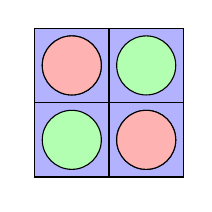
\begin{tikzpicture}[scale=0.75, every node/.style={scale=1}]
        \foreach \x in {0,1.26}
        \foreach \y in {0,1.26}
        \filldraw[xshift=\x cm, yshift=\y cm, fill=blue!30!white, 
        draw=black] (0, 0) rectangle (1.26,1.26) node[pos=.5] {};
        \foreach \x in {0,1.26}
        \foreach \y in {0,1.26}
        \filldraw[xshift=\x cm, yshift=\y cm, fill=green!30!white, 
        draw=black] (.63,.63) circle (.5) node[pos=.5] {};
        \filldraw[xshift=0 cm, yshift=1.26 cm, fill=red!30!white, 
        draw=black] (.63,.63) circle (.5) node[pos=.5] {};
        \filldraw[xshift=1.26 cm, yshift=0 cm, fill=red!30!white, 
        draw=black] (.63,.63) circle (.5) node[pos=.5] {};
    \end{tikzpicture}
    \caption{Configuration for pincell junction; all Reflect BC; Every 
        combination is used}
    \label{fig:junction_config}
\end{figure*}

The next model was to create a small version of the C5G7 core, which 
has the same assembly configuration shown in \FIG{fig:C5G7_config}, but 
instead uses 8-pin by 8-pin assemblies.  The small UO$_2$ assembly is shown in 
\FIG{fig:small_UO2}, and the small MOX assembly is shown in  
\FIG{fig:small_MOX}. 

\begin{figure*}[htb]
    \centering
    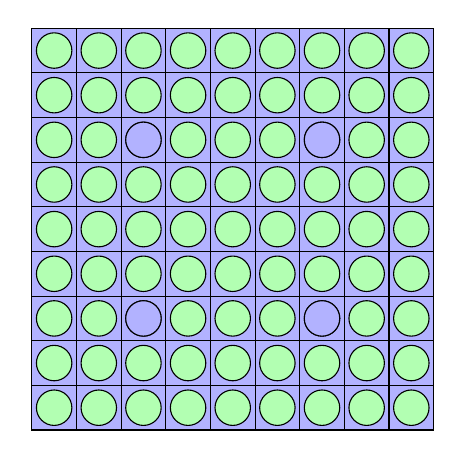
\begin{tikzpicture}[scale=0.45, every node/.style={scale=1}]
        \foreach \x in {0,1.26,...,10.08}
        \foreach \y in {0,1.26,...,10.08}
        \filldraw[xshift=\x cm, yshift=\y cm, fill=blue!30!white, 
        draw=black] (0, 0) rectangle (1.26,1.26) node[pos=.5] {};
        \foreach \x in {0,1.26,...,10.08}
        \foreach \y in {0,1.26,...,10.08}
        \filldraw[xshift=\x cm, yshift=\y cm, fill=green!30!white, 
        draw=black] (.63,.63) circle (.5) node[pos=.5] {};
        \foreach \x in {2*1.26, 6*1.26}
        \foreach \y in {2*1.26, 6*1.26}
        \filldraw[xshift=\x cm, yshift=\y cm, fill=blue!30!white, 
        draw=black] (.63,.63) circle (.5) node[pos=.5] {};
    \end{tikzpicture}
    \caption{Configuration for small UO$_2$ fuel bundle.  The green represents 
             a UO$_2$ pincell, while the blue represents a guide tube modeled 
             as a pincell filled with moderator}
    \label{fig:small_UO2}
\end{figure*}
\begin{figure*}[htb]
    \centering
    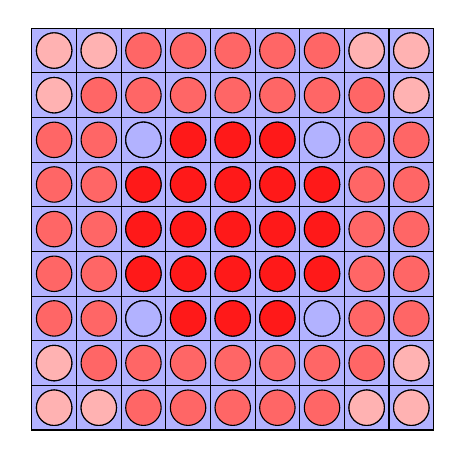
\begin{tikzpicture}[scale=0.45, every node/.style={scale=1}]
        \foreach \x in {0,1.26,...,10.08}
        \foreach \y in {0,1.26,...,10.08}
        \filldraw[xshift=\x cm, yshift=\y cm, fill=blue!30!white, 
        draw=black] (0, 0) rectangle (1.26,1.26) node[pos=.5] {};
        \foreach \x in {0,1.26,...,10.08}
        \foreach \y in {0,1.26,...,10.08}
        \filldraw[xshift=\x cm, yshift=\y cm, fill=red!60!white, draw=black] 
        (.63,.63) circle (.5) node[pos=.5] {};
        \foreach \x in {0,1.26,7*1.26,10.08}
        \foreach \y in {0,10.08}
        \filldraw[xshift=\x cm, yshift=\y cm, fill=red!30!white, draw=black] 
        (.63,.63) circle (.5) node[pos=.5] {};
        \foreach \x in {0,10.08}
        \foreach \y in {1.26,7*1.26}
        \filldraw[xshift=\x cm, yshift=\y cm, fill=red!30!white, draw=black] 
        (.63,.63) circle (.5) node[pos=.5] {};
        \foreach \x in {2.52,3.78,...,7.56}
        \foreach \y in {2.52,3.78,...,7.56}
        \filldraw[xshift=\x cm, yshift=\y cm, fill=red!90!white, draw=black] 
        (.63,.63) circle (.5) node[pos=.5] {};
        \foreach \x in {2*1.26, 6*1.26}
        \foreach \y in {2*1.26, 6*1.26}
        \filldraw[xshift=\x cm, yshift=\y cm, fill=blue!30!white, 
        draw=black] (.63,.63) circle (.5) node[pos=.5] {};
    \end{tikzpicture}
    \caption{Configuration for small MOX bundle.  The light red represents 
             4.3\% MOX fuel, the medium red represents 7.0 \% MOX fuel, and the 
             dark red represents 8.7\% MOX fuel.  The blue represents 
             moderator, light water}
    \label{fig:small_MOX}
\end{figure*}

An additional model arises from the small core model, which is to 
combine snapshots from each of the small assemblies.  This is not expected to 
perform as well as the full-sized, combined-assembly model, but it will be 
quicker to create the snapshots, and thus the basis functions.  A third model 
from the small core was to spatially average the snapshots for each pincell 
similarly to the spatially-reduced, full-core solution.  The reduced, small-core 
model was used to approximate the non-spatially averaged, full-core 
model by comparing the reduced and non-reduced small-core models.  

The final snapshot model for the C5G7 test problem is to create a 
similar 1-D model.  This is shown in \FIG{fig:1D_C5G7}.  The model is 
comprised of 51 pins that are each of width 1.26 cm.  The fuel section for each 
pin was modeled at 1.08 cm, leaving 0.09 cm of moderator on either side.  This 
problem was created with a reflective boundary condition on the UO$_2$ side of 
the model and a vacuum boundary condition on the moderator side of the model.

\begin{figure*}[htb]
    \begin{minipage}[c]{\textwidth}
        \centering
        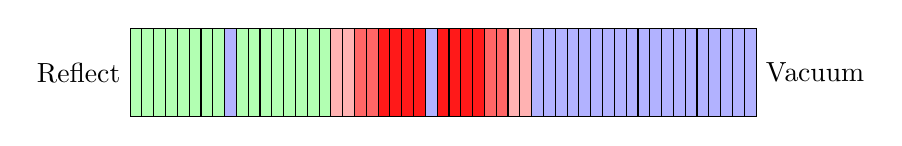
\begin{tikzpicture}[scale=1.5, every node/.style={scale=1}]
            \foreach \x in {0,.1,...,1.7}
            \filldraw[xshift=\x cm,fill=green!30!white,draw=black] (0,0) 
            rectangle (0.1,.75);
            \foreach \x in {1.7,1.8,...,3.4}
            \filldraw[xshift=\x cm,fill=red!30!white,draw=black] (0,0) 
            rectangle (0.1,.75);
            \foreach \x in {1.9,2.0,...,3.2}
            \filldraw[xshift=\x cm,fill=red!60!white,draw=black] (0,0) 
            rectangle (0.1,.75);
            \foreach \x in {2.1,2.2,...,2.9}
            \filldraw[xshift=\x cm,fill=red!90!white,draw=black] (0,0) 
            rectangle (0.1,.75);
            \foreach \x in {3.4,3.5,...,5.3}
            \filldraw[xshift=\x cm,fill=blue!30!white,draw=black] (0,0) 
            rectangle (0.1,.75);
            \foreach \x in {0.8,2.5}
            \filldraw[xshift=\x cm,fill=blue!30!white,draw=black] (0,0) 
            rectangle (0.1,.75);
            \draw (5.3,.375) node[right] {Vacuum};%
            \draw (0,.375) node[left] {Reflect};
        \end{tikzpicture}
    \end{minipage}
    \begin{minipage}[c]{\textwidth}
        \centering
        \vspace*{-.05cm}
        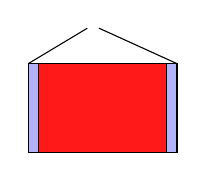
\begin{tikzpicture}[scale=1.5, every node/.style={scale=1}]
            \draw (0,.75) -- (.5,1.05) (.6,1.05) -- (1.26,.75);
            \filldraw[xshift=0 cm,fill=blue!30!white,draw=black] (0,0) 
            rectangle (.09,.75);
            \filldraw[xshift=.09 cm,fill=red!90!white,draw=black] (0,0) 
            rectangle (1.17,.75);
            \filldraw[xshift=1.17 cm,fill=blue!30!white,draw=black] (0,0) 
            rectangle (.09,.75);
        \end{tikzpicture}
    \end{minipage}
    \caption{Configuration for 1D approximation to the C5G7 benchmark.  The 
             green represents UO$_2$, the light red represents 
             4.3\% MOX fuel, the medium red represents 7.0 \% MOX fuel, and the 
             dark red represents 8.7\% MOX fuel, and the blue 
             represents moderator}
    \label{fig:1D_C5G7}
\end{figure*}

\section{SERMENT and DETRAN}

All of the solvers and methods, save for new basis generation, were developed 
previously and implemented in two transport codes, DETRAN and SERMENT.   The SERMENT parallel 
response matrix  code 
\citep{RobertsSerment} links to the DETRAN deterministic transport 
code \citep{RobertsDetran} to implement ERMM and allows the choice of several 
orthogonal basis sets.  DETRAN implements discrete ordinates, method of 
characteristics, and diffusion approximations, along with several advanced 
solvers developed specifically for use in response function generation. For 
this 
work, only its discrete ordinates capabilities were used.

DETRAN was used to generate the data to be used for each of the snapshot 
models.  It requires no basis expansions, 
and is taken as the true solution for each of the test problems.  SERMENT 
was used to generate the reference case for each test problem against which all of 
of the KLT solutions for the given test problem were compared.  The reference 
case was taken as a full order multi-group approximation with the same spatial 
and angular expansions as the KLT cases.  This was done to isolate the error 
caused by the expansion in energy to the greatest extent possible.  

The new functionality for SERMENT that was developed in this work is the 
ability to incorporate user-defined basis sets.  This allows an arbitrary order 
and size of basis functions to be passed to SERMENT enabling expansion 
via that basis.  